\section{Modeling requirements}

\begin{definition}
    A \emph{model} is a depiction, typically in one medium, of an entity in the same or a different medium.
    It encapsulates the essential facets of the subject while simplifying or omitting extraneous details.
\end{definition}
Reality, denoted as $R$, comprises tangible entities, individuals, processes, and their interconnections. 
In contrast, a model, symbolized as $M$, represents an abstraction of these entities, individuals, processes, and the relationships between these abstractions.

To comprehend reality, it necessitates interpretation denoted as $I$ through a mapping function.
For a model to be considered effective, it is imperative that the relationships that hold true in reality $R$ also hold true in the model $M$.
\begin{figure}[H]
    \centering
    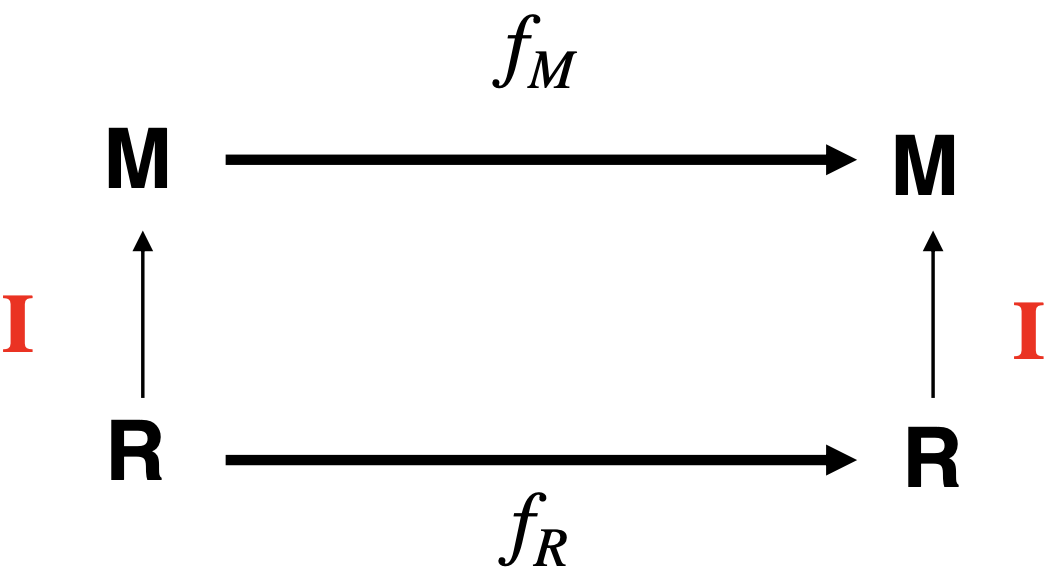
\includegraphics[width=0.35\linewidth]{images/modeling.png}
    \caption{Relationship between model $M$ and reality $R$}
\end{figure}
Software models serve a variety of purposes, including:
\begin{itemize}
    \item Capturing and articulating requirements and domain knowledge with precision.
    \item Facilitating software system design and the generation of practical deliverables.
    \item Offering a simplified perspective on intricate systems and enabling evaluation and simulation of such complexity.
    \item Generating prospective system configurations.
\end{itemize}
The primary modeling challenges revolve around ensuring coherence among different perspectives of the system and addressing the potential for variations in interpretation and ambiguity by establishing clear boundaries for acceptable differences in how the model is understood.
 
In the domain of requirements engineering, our modeling efforts should primarily focus on:
\begin{itemize}
    \item Representing the pertinent entities and individuals relevant to the given problem.
    \item Describing the relevant phenomena.
    \item Documenting the objectives, requirements, and domain assumptions.
\end{itemize}
When it comes to choosing the appropriate modeling tools, we have several options at our disposal:
\begin{itemize}
    \item Natural language (e.g., English, Italian, etc.):
        \begin{itemize}
            \item Pros: user-friendly and easy to use.
            \item Cons: prone to a high level of ambiguity, and it's possible to overlook relevant information.
        \end{itemize}
    \item Formal language (e.g., FOL, Alloy, Z, etc.):
        \begin{itemize}
            \item Pros: offers the possibility of employing tools for analysis and validation; this approach compels the user to specify all crucial details.
            \item Cons: requires expertise in using the language.
        \end{itemize}
    \item Semiformal language (e.g., UML):
        \begin{itemize}
            \item Pros: simpler than a formal language, providing some degree of structure to the models.
            \item Cons: not amenable for automated analysis, and still entails some level of ambiguity.
        \end{itemize}
    \item Mixed approach:             
        \begin{itemize}
            \item Utilizing a semiformal language for foundational aspects.
            \item Augmenting semiformal models with explanatory informal text.
            \item Leveraging a formal language for the most critical components.
        \end{itemize}
\end{itemize}
The choice of the modeling tool should align with the specific requirements and characteristics of the project at hand.